%%%%%%%%%%%%%%%%%%%%%%%%%%%%%%%%%%%%%%%%%%%%%%%%%
%%%%%%%%%%%%%%%%%%%%%%%%%%%%%%%%%%%%%%%%%%%%%%%%%

\chapter{Nature-based Algorithms for Prioritized Foraging}
\label{chap:third}

%%%%%%%%%%%%%%%%%%%%%%%%%%%%%%%%%%%%%%%%%%%%%%%%%
%%%%%%%%%%%%%%%%%%%%%%%%%%%%%%%%%%%%%%%%%%%%%%%%%

%The same structure as before, including section, subsections and sub-subsections. Make sure that you follow the same conventions throughout, to avoid confusing the reader. Always remember to include a summary.

%%%%%%%%%%%%%%%%%%%%%%%%%%%%%%%%%%%%%%%%%%%%%%%%%
%%%%%%%%%%%%%%%%%%%%%%%%%%%%%%%%%%%%%%%%%%%%%%%%%

\section{Na\"ive Foraging Algorithm}

%Need to expand over here lots. Add formulas for each one and pictures.
%Describe specific implementation. 1hr to regather research for specific technique. 0.5 - 1.5 to document what happened in the code. Per technique

Naive foraging is used as a lower bound for comparison as is done in \cite{62} \cite{63}. Na\"\i ve foraging includes only the most minimal set of foraging actions. Na\"\i ve foraging is included as a baseline for comparison to evaluate how a memory-based technique such as desert-ant foraging compares to a standard model \cite{ostergaard2001emergent,hoff2010two}.

 Na\"\i ve foraging consists of the following tasks: searching for an item, grabbing an item, returning home with the item and storing the item at the sink as shown in Figure \ref{naiveforagestate}. The robots repeat the following steps: 

\begin{enumerate}
	\item Robots perform a random walk until they find an item.
	\item On locating an item, the robot grips the item. If the item has been moved before the robot is able to pick it up, the robot will continue to explore; otherwise the robot returns the item to the correct sink using a beacon-based homing algorithm.
\end{enumerate}
\begin{figure}
	\centering
	\includegraphics[width=0.55\textwidth]{diagrams/NaiveForaging.pdf}
	\caption{Na\"ive Foraging State Diagram}
	\label{naiveforagestate}
\end{figure}

The following random walk is used: A robot chooses a random direction, $\sigma$, and a random distance $m\in(0,M)$ where $M$ is a chosen maximum path length. The robot walks in direction $\sigma$ for distance $m$. The robot then chooses new values for $\sigma$ and $m$. 


\subsection{Desert Ant Foraging}

Due to the lack of pheromone, desert ant foraging behaviour is a very suitable model for robot foraging. Desert ants use path integration to memorize the location of an existing food source and later to return to the memorized source to find more food. The notion of returning to a previously explored site is known as site fidelity \cite{switzer1993site}. The desert ant algorithm does not require communication between robots or the dispersal of beacons, and is thus simpler than other many swarm robotics foraging algorithms. 

Path integration (PI) is the integration of an ant's odometry such that the ant can maintain a position and heading estimate of where the ant is going, by continuously updating a heading direction vector that points to the starting position \cite{ronacher2008path}. The heading-direction vector is known as the PI vector. This type of behaviour theoretically appears suitable for environments where multiple items occur in similar areas. The disadvantage of PI is the accumulation of localisation errors. The robot control algorithm consists of five states ( illustrated in Fig \ref{fig:desertantstate}):

\begin{enumerate}
	\item\textbf{Exploration} -- the robot performs a random walk while performing PI.
	\item\textbf{Loading} -- on finding an item, the robot loads the item and memorizes the PI vector.
	\item\textbf{Homing } -- the robot uses the path integration vector to move to the sink.
	\item\textbf{Off-loading} -- when the robot is at the sink, the object is offloaded.
	\item\textbf{Locating} -- the robot follows the memorized PI vector to the location of the previous item. If another item is found, the item is loaded; otherwise the robot returns to the exploration state. 
\end{enumerate}
All robots begin at random positions adjacent to the sink in the exploration state.

\begin{figure}[h]
	\centering
	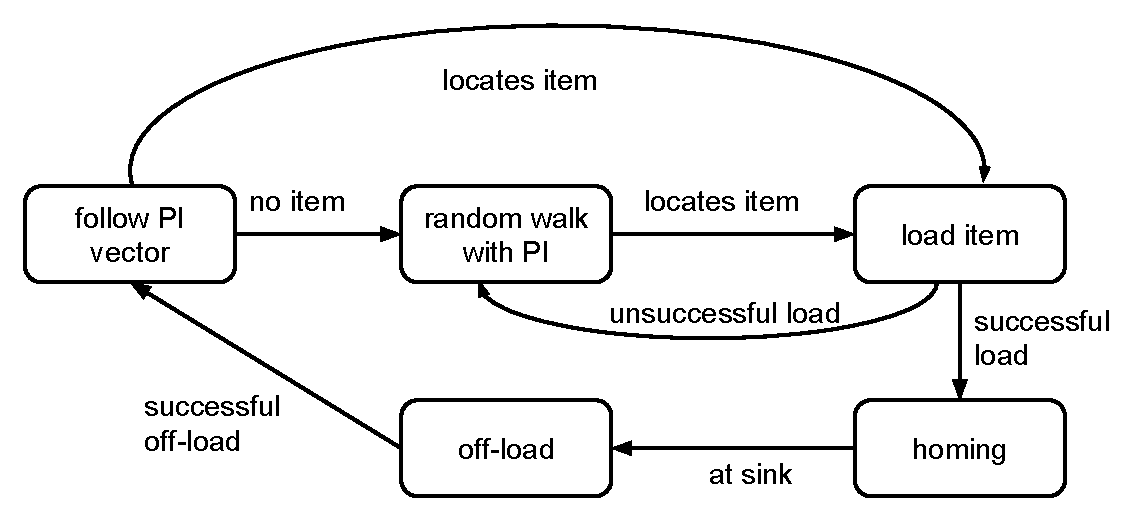
\includegraphics[width=0.75\textwidth]{diagrams/DesertAntState.pdf}
	\caption{Desert Ant Foraging State Diagram}
	\label{fig:desertantstate}
\end{figure}
	
%%%%%%%%%%%%%%%%%%%%%%%%%%%%%%%%%%%%%%%%%%%%%%%%%
%%%%%%%%%%%%%%%%%%%%%%%%%%%%%%%%%%%%%%%%%%%%%%%%%

\subsection{Honey Bee Foraging}

The presented honey bee algorithm is based on the mathematical model of honey bee foraging in \cite{seeley2009wisdom}. A portion of the robots are initialized as scouts and the rest  as unemployed foragers in a waiting state. All robots are initialized adjacent to the item sinks.

Fig \ref{honeybeestate} is a simplified state diagram for the honey bee algorithm. State transitions are described as follows: 

\begin{enumerate}

\item A scout robot performs a random walk and, upon finding an item and evaluating the site, forages the item by returning the item to the sink using PI. 

\item A scout decides to dance, based on the quality of the site. If the estimated quality of the site, $\mu$, is less than the dance threshold, $\phi$, the scout robot does not dance and instead continues to forage the site as an employed forager.

\item Otherwise, if the estimated quality of the site, $\mu$, is greater or equal to the dance threshold, $\phi$, the scout robot dances for the unemployed foragers.

\item After a dance is complete, the scout robot decides with probability $\rho$ to start exploring again or recruit itself and begins foraging the found site.

\item On detecting a dance, waiting bees become foraging bees with a probability $\alpha$ and switch to foraging the dancer's item type.

\item Employed foragers become unemployed foragers (waiting foragers) if the foraging site has been depleted.

\item Unemployed foragers become scouts if no dances are detected $t_{max}$ time steps.

\end{enumerate}

\begin{figure}[h]
	\centering
	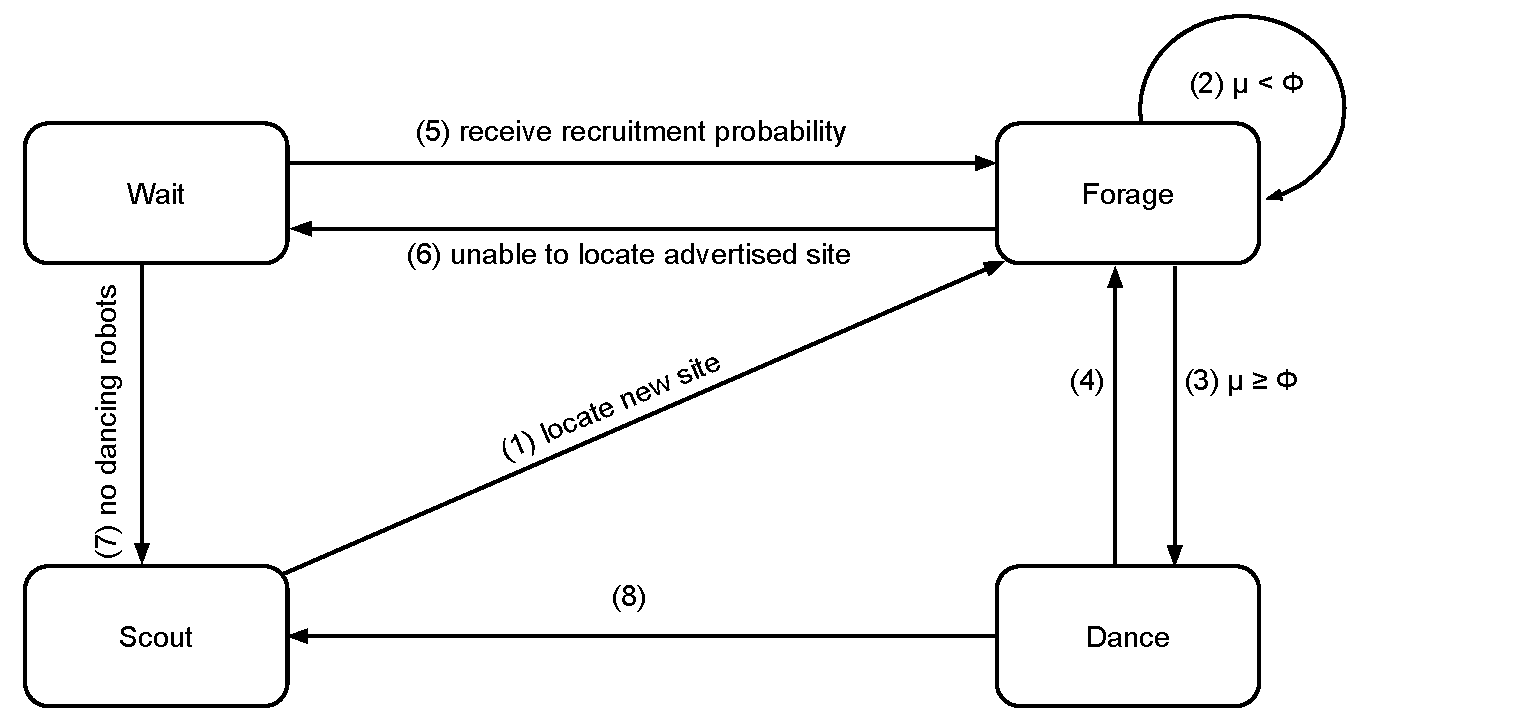
\includegraphics[width=0.75\textwidth]{diagrams/HoneyBee.pdf}
	\caption{Honey Bee Foraging State Diagram }
	\label{honeybeestate}
\end{figure}

Site quality, $\mu_t$, for a robot scouting items of type $t$, is calculated as the estimated density of items of type $t$ in the local vicinity of the found item. The robot has distance sensor values $k_i\in[0,1]$ for $ i = 1...n$, where 0 means that nothing is detected in sensor range and 1 indicates that the robot is touching an item and $n$ is the number of distance sensors. The item density of type $t$, $\mu_t$, is calculated using
\begin{equation}
\label{density}
\mu_t = \frac{1}{n}\sum\limits_{i=1}^n k_{i_t}
\end{equation}
where the sensor value for item type $t$, $k_{i_t}$, is calculated using 
\begin{equation}
\label{densitytype}
k_{i_t}=
    \begin{cases}
      k_i & \text{if item $i$ is type $t$} \\
      0 & \text{otherwise}
    \end{cases}
\end{equation}

In nature, in times of drought, bees prioritize water over nectar or pollen. Bees are sent out to forage water; however, if they happen to encounter pollen, they will forage it but will not communicate the discovery to the unemployed foragers  \cite{seeley2009wisdom}. The rules for item-type division of labour are based on the behaviour of bees under environmental pressure as follows:

\begin{enumerate}
\item A robot foraging the prioritized type, forages a non-prioritized type only if a prioritized item can not be located for max time $f_{max}$.
\item A robot foraging a non-prioritized item forages the non-prioritized item type until the robot fails to relocate the site or the robot locates a prioritized item. The robot switches to foraging the prioritized item.
\item A robot foraging a non-prioritized item will not communicate the location of the non-prioritized item site by dancing. 
\end{enumerate}

For the purpose of this study, honey bee robots are initialized to start foraging a particular item type to show the effectiveness of the division of labour. The presented algorithms differ in three main properties as given in Table \ref{properties}.

\subsection{Summary}
\begin{table} [h]
    \caption{Properties of the foraging algorithms used in this study}
    \label{properties}
	\centering
    \begin{tabular}{|l|c c c|} \hline
    Property           & Na\"ive  & Desert Ant  & Honey Bee  \\ \hline
    Memory             & \xmark  & \cmark     & \cmark    \\
    Communication      & \xmark  & \xmark     & \cmark    \\
    Division of Labour & \xmark  & \xmark     & \cmark    \\ \hline
    \end{tabular}

\end{table}


\section{Navigation and Obstacle Avoidance}
\label{thri:third:obstacleavoidance}

\subsection{Navigation and Obstacle Avoidance}
Due to the complexity of the environments, an advanced navigation and obstacle avoidance technique is required.  The technique is based on the flocking behaviour of birds used in \cite{antoniou2012congestion}.

The force that pulls the birds to the destination is known as the global attractor, while a local attractor is a force that directs birds away from local obstacles. As a result birds avoid local obstacles while maintaining course to the destination. 

Figure \ref{fig:obstacleavoidance} illustrates the obstacle avoidance method used by the agents. The obstacle avoidance algorithm achieves the effect of the global attractor by setting the robots field of view towards the direction to the desired destination. The destination is determined by a homing beacon or by the robot's path integration. The direction at the centre of the field of view is the direction to the destination. 

The effect of the local attractor is modelled by evaluating a function for each direction in the field of view, and the most desirable direction is chosen. Desirability, $d$, is defined as a path that achieves an adequate balance between clarity and directness. Clarity id direction $i$, $c_i$, is a normalized proximity sensor or camera reading in the range (0,1) indicating the distance of next nearest obstacle where 0 occurs if no obstacles exist in the destination for the depth of view $v$. The directness of a direction $i$, $\tau_i$, occurs in the range (0,1) and is calculated as the angular deviation from the direction of the destination, where 0 is achieved when the direction $i$ is the same as direction to the destination and 1 occurs when the direction is at the edge of the field of view, $f$. Desirability $d_i$ of direction $i$ is defined mathematically in Equation \ref{eq:1}.

\begin{equation}
	d_i= \lambda c_i + (1 - \lambda)\tau_i \\
	\label{eq:1}
\end{equation} where $\lambda$ determines whether clarity, $c_i$ or directness, $\tau_i$ of direction $i$, has more effect.
 
The described navigation and obstacle avoidance technique is used with all algorithms in the experiment and for algorithms $\lambda$ is set to 0.5.

\begin{figure}
	\centering
	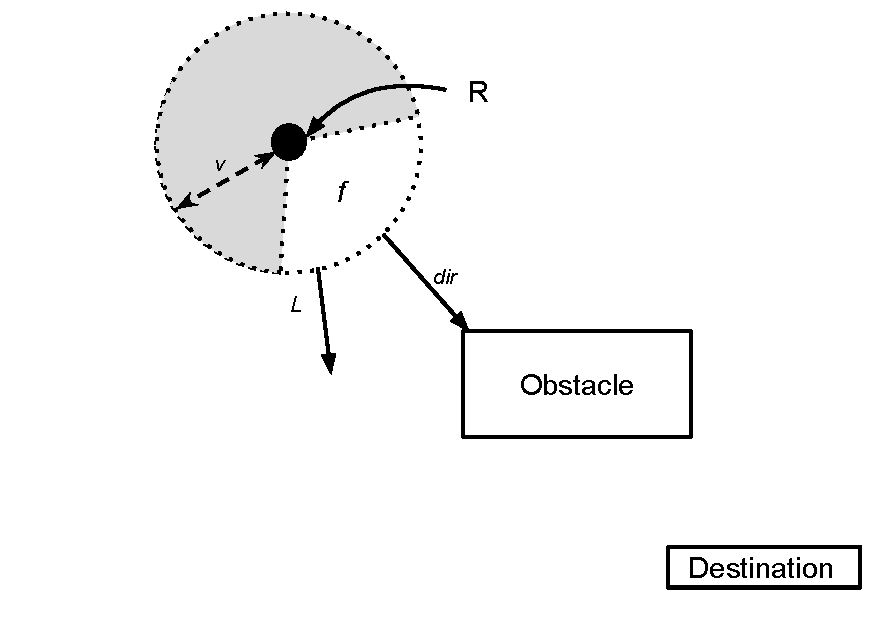
\includegraphics[width=0.5\textwidth]{chapters/chapter3/figures/ObstacleAvoidance.pdf}
	\caption{Obstacle Avoidance. $v$ is depth of view, $f$ is field of view, $R$ is the robot, $dir$ is the direction of the destination, $L$ is a possible value of local attractor}
	\label{fig:obstacleavoidance}
\end{figure}


\section{Model Description}

\subsection{Na\"\i ve Foraging}

 Na\"\i ve foraging includes only the most minimal set of foraging actions. Na\"\i ve foraging is included as a baseline for comparison \cite{hoff2010two} \cite{ostergaard2001emergent} in order to evaluate how a memory-based technique such as desert-ant foraging compares to a standard model.

 Na\"\i ve foraging consists of searching for an item, grabbing an item, returning home with the item and storing the item at the store house. The robots repeat these steps. 

Define a random walk. \cite{54}
\begin{itemize}
	\item Robots perform a random walk until they find item.
	\item On locating an item, the robot grips or picks-up the item. In the case where the item has been moved before the robot is able to pick it up, the robot will continue to explore otherwise the robot returns the item to the correct sink.
\end{itemize}
\begin{figure}
	\centering
	\includegraphics[width=0.5\textwidth]{chapters/chapter3/figures/NaiveForaging.pdf}
	\caption{Na\"ive Foraging State Diagram}
\end{figure}



Due to the variety of environments that the algorithms are being experimented on, sophisticated navigation and obstacle avoidance is required. All algorithms use the same navigation and obstacle avoidance techniques when 
%%%%%%%%%%%%%%%%%%%%%%%%%%%%%%%%%%%%%%%%%%%%%%%%%
%Don't think this goes here
%Provide equations for each one. Should take about 15 - 20 minutes per equation. 

%%%%%%%%%%%%%%%%%%%%%%%%%%%%%%%%%%%%%%%%%%%%%%%%%
%%%%%%%%%%%%%%%%%%%%%%%%%%%%%%%%%%%%%%%%%%%%%%%%%
\section{Summary}
\label{sec:second:summary}

%%%%%%%%%%%%%%%%%%%%%%%%%%%%%%%%%%%%%%%%%%%%%%%%%
%%%%%%%%%%%%%%%%%%%%%%%%%%%%%%%%%%%%%%%%%%%%%%%%%